\section{Inferencia da EADS}
Um grande problema para modelos que utilizam de aprendizado é a recorrência de dados, isso por que uma amostra com dados coletados de maneira incorreta pode resultar em \textit{overfitting}\footnote{Termo utilizado para quando a máquina fica "viciada" apenas a um dado, sendo muito boa em resolver os dados do \textit{dataset} inicial mas perdendo eficiencia em novos dados} ou até mesmo em um baixa acertividade. No caso os dados coletados são suficientes para provar a teoria de inferencia, porém, o dataset conta com aproximadamente 620 linhas, é um número relativamente baixo para ensinar uma máquina. Outro problema é a falta de consistência entre as questões. Existem questões como muito \textit{support}\footnote{Termo para dados que suportaram os resultados, quanto mais dados apresentados para uma certa ocasião, maior o suporte do modelo para aquele tipo de dado}, entretanto, exitem dados com baixo fluxo de respostas (incluindo a questão "Minha boca ficou seca" que não teve uma única resposta).

Para provar o conceito, será utilizado o algoritmo Gaussian do Naive Bayes\cite{john1995estimating}. Dentro do Python existe uma biblioteca chamada Sklearn\footnote{\url{}}, ela já trás diversos algoritmos de aprendizagem para submeter o conjunto de dados para aprendizagem e posteriormente para análise. Com o banco devidamente anotado e processado é possível utilizar um outro \textit{script}, vindo da biblioteca em \textbf{go}, para extrair os dados de predição do banco para dentro do 14BIS.

O código de extração foi baseado na teoria do \textit{Bag of Words}\cite{zhang2010understanding}, em outras palavras, é baseado em utilizar toda a palavra, do texto normalizado, como um atribudo a ser estudado pela maquina. Na linha do dado é marcado a quantidade de vezes que aquele atributo (no caso a palavra), apareceu na frase. Por mais que seja uma abordagem é possível notar estudos como o de Bharath Sriram que diz sobre algumas limitações da abordagem, principalmente a escalabilidade infinita dependendo da quantidade de dados e diferentes palavras apresentadas \cite{sriram2010short}. Vale lembrar que qualquer "sujeira" textual que passe durante a normalização do dado pode afetar o resultado.

É possível achar o código da aprendizagem em \textit{14bis/src/question\_model.py}\footnote{Código no GitHub: \url{}}, é utilizado o padrão do Sklearn junto com o JSON gerado pelo \textit{script} em \textbf{go} responsavel no intercâmbio dos dados do banco para um arquivo unificado. Ao observar a Figura \ref{fig:prediction} é possível notar que a precisão da questão 2 (com a maior quantidade de suporte é de 1.0 e seu \textit{recall}\footnote{Margem dada por falsos positivos} é de apenas 0.2), enquanto dados com menor número de suporte tendenciam a ter o mesmo \textit{recall} maior e precisão menor. Por esses motivos por mais que a precisão da maquina esteja em 60\% o \textit{recall} esta tão alto quanto chegando aos 44\%.

\begin{figure}[!ht]
    \centering
    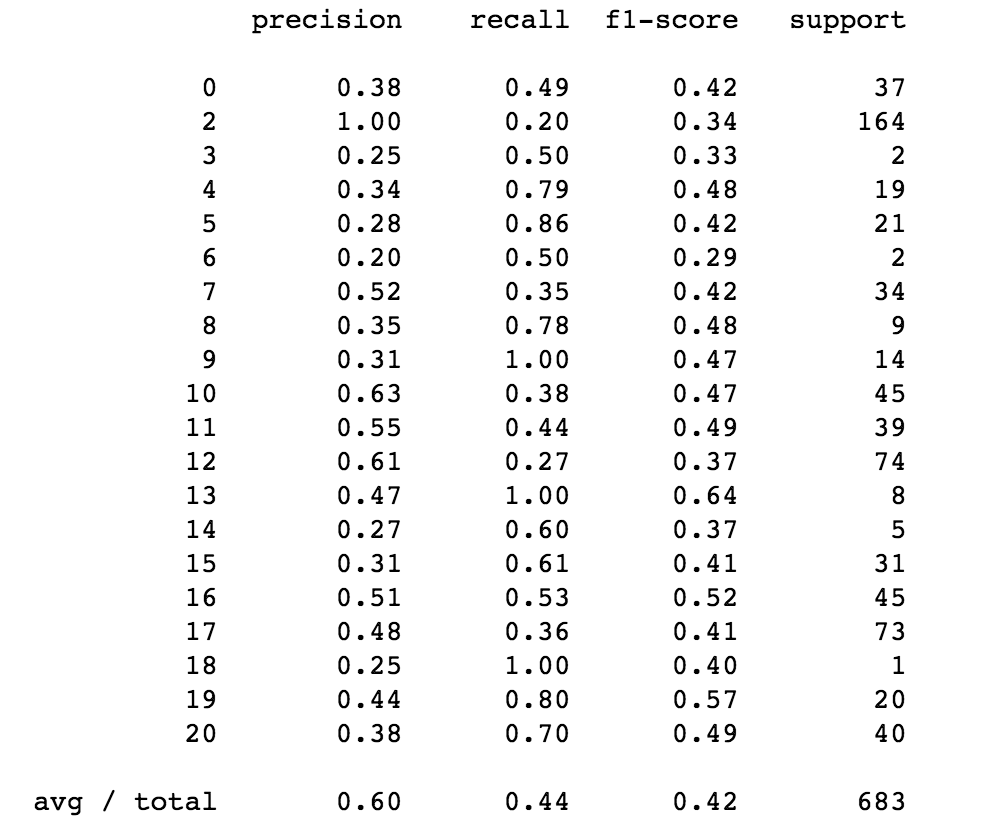
\includegraphics[width=.6\textwidth]{imagens/prediction.png}
    \caption{Tabela de resultados do Naive Bayes para 683 resultados}
    \label{fig:prediction}
\end{figure}

Com isso é possível concluir que é factivel predizer questões da EADS, porém, mais dados precisam ser recolhidos e novas abordagens podem ser textadas para refinar o modelo e melhorar sua \textit{performance}.

Dando sequencia, caracterizar dimensões afetivas negativas através de EADS é algo relativamente simples uma vez que o usuário responda o teste, existem operações matemáticas que podem ser rapidamente aplicadas em cima dos dados para gerar a informação proposta pela ferramenta. Já foi observada a possibilidade de inferencia nas questões, entretanto, a dicussão agora é puxada para contexto agrupado, ou seja, a escala em si. Quando foi proposto uma IA entender esse usuário e simular o preenchimento dessa escala baseado em suas publicações alguns problemas podem ser notados:

\begin{itemize}
    \item A recorrência, ou seja, como analisar que um estado obtido por uma publicação perdura ou se foi algo meramente momentâneo, assim como se essa discrepância afeta no impacto da resposta (se aplica ou não a pessoa).
    \item A presença de dimensões, em outras palavras, se a pessoa realmente se expressa pelo Twitter, existem casos que pessoas podem ser mais introspectivas.
    \item Efeitos Colaterais, no caso em que nem todas as perguntas sejam respondidas, existiria algum padrão para ponderar e inferir as perguntas não preenchidas.
\end{itemize}

Para isso foi solicitado a ajuda de  de nove usuário, sendo que seus nomes serão omitidos por conta da privacidade. No Twitter para que fosse monitorada sua atividade por uma semana, no final desse prazo foi aplicado a EADS via Google Forms. Os tweets passaram pelo mesmo processo de mineração dos tweets coletados por palavras chaves, entretanto, o foco nesse momento era na segunda parte da proposta, caracterizar as dimensões afetivas. O primeiro passo foi separar desses 9 perfis, os perfis que tinham potenciais de demonstrar algum dado que viabilizasse a construção de um modelo. A partir da média de 23 perguntas, foi separado qualquer perfil que atendesse a esses requisitos, e foram localizados 3 perfis. Ao observar a Figura \ref{fig:ueadsr} é possível notar os valores da EADS respondidas pelos usuários (0), (1) e (2).

\begin{figure}[!ht]
    \centering
    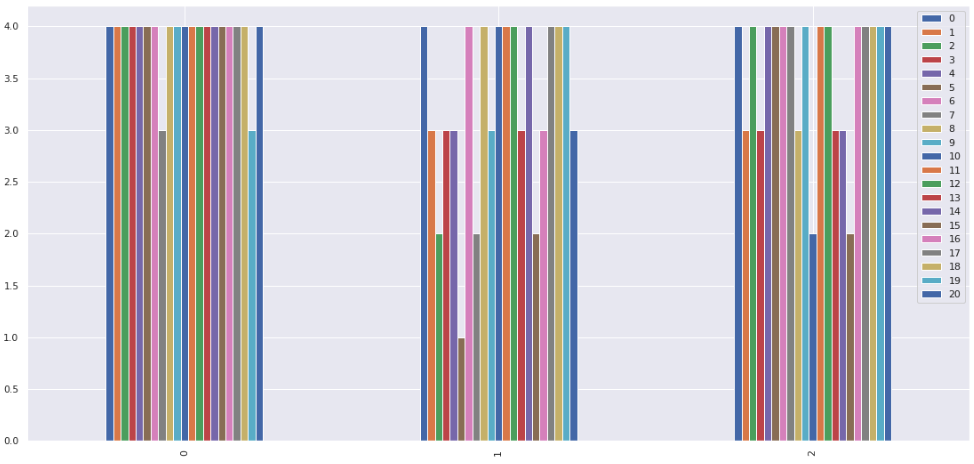
\includegraphics[width=1\textwidth]{imagens/ueadsr.png}
    \caption{Demonstração grafica da EADS de uma amostra de 3 usuários}
    \label{fig:ueadsr}
\end{figure}

O próximo passo era localizar uma possível relação entre a frequência de postagens e as escalas, entretanto, devido a movimentações da semana, alguns dias aparecem sem publicações. Logo a segunda solução foi procurar algo relativo a quantidade de perguntas respondidas na semana. Ao observar a solução de uma escala Likert, modelo no qual a EADS é baseada, pode-se notar que algumas médias são retiradas isolando valores em grupos maiores, em outras palavras criando grupos que agreguem uma quantidade de subvalores para pode retirar uma média de maneira mais assertiva. Escalas Likert podem ter N valores, no caso da EADS ela é composta por apenas 4, logo ela seria divida em 1 e 2 sendo os menos aplicados e 3 e 4 como os mais aplicados. A partir disso se passa-se a observar primeiramente apenas 2 repartições. Baseado nisso é possível analisando a Figura \ref{fig:table}, notar que as maiores quantidades de respostas provem dos itens localizados entre 3 e 4 na escala, porém, existem algumas exceções, como por exemplo, dados que estão presentes na escala porém não são referenciados por tweets. Isso como já foi mostrado em análises posteriores se deve a raramente o usuário expressar algumas ações como tremedeira, pré ataque de pânico, falta de saliva e outros recursos físicos apresentados na tabela. Entretanto, mais uma vez, pode-se afirmar que a correlação interna dos itens e a externa pelos constructos (ansiedade, depressão e stress), podem ser uma espécie de ativador na criação do modelo, uma vez que a existencia de um item possa influenciar na aparição de um outro.

\begin{figure}[!ht]
    \centering
    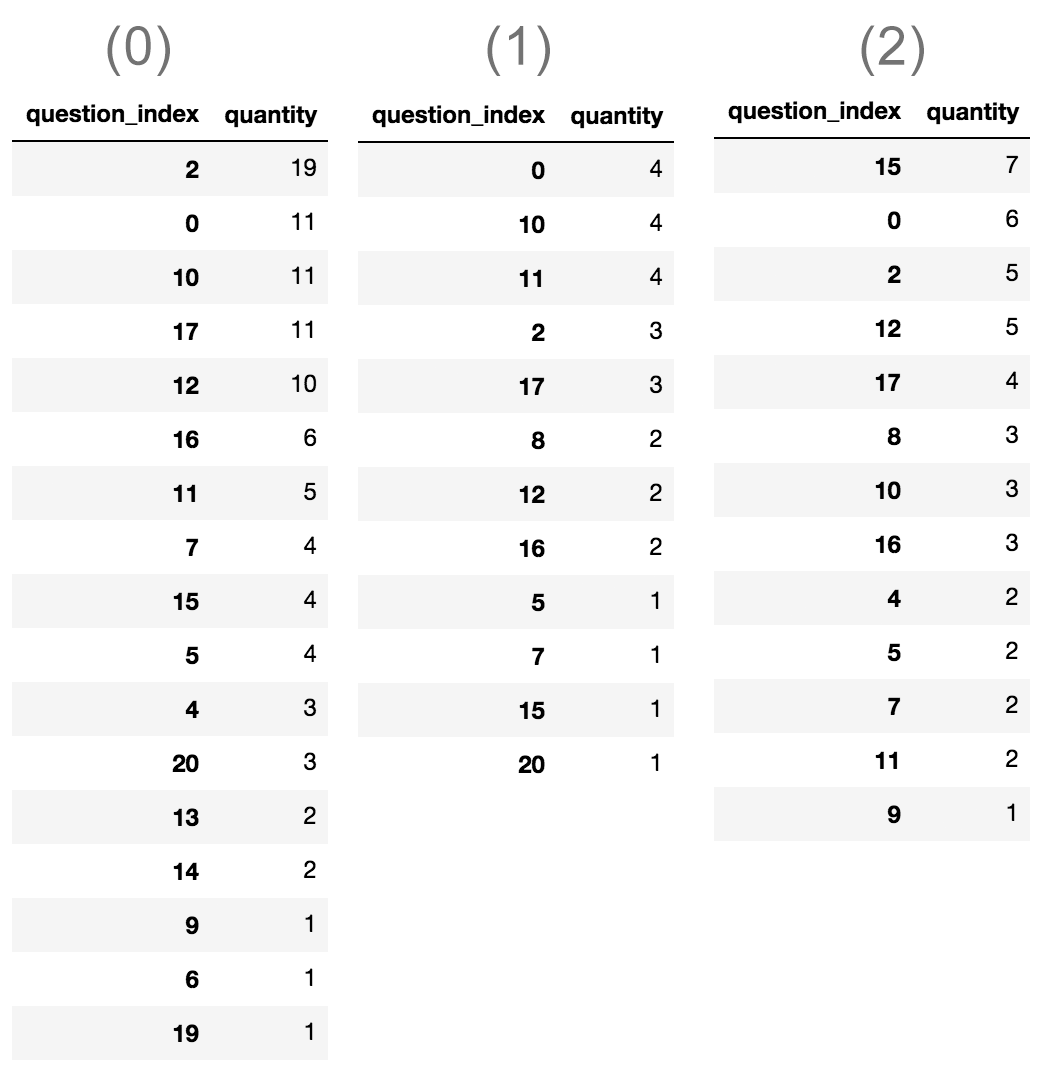
\includegraphics[width=.6\textwidth]{imagens/table.png}
    \caption{Tabela de Questões da EADS respondidas pelos 3 usuários durante a semana}
    \label{fig:table}
\end{figure}

Infelizmente a quantidade de dados impossibilita a criação e teste de um modelo, além de, afirmações mais insicivas como a questão de quais itens poderiam influenciar na aparição de outros. Logo não foi possível gerar um modelo mas foi possível idealizar problemas e localizar pontos para futuras explorações gerando alguns resultados e discussões interessantes sobre o assunto.